\pdfminorversion=6 % this is needed to be able to include pdf 1.6. 
                    % For some reasons some old HPSG proceedings have pdf 1.6
\documentclass[11pt,a4paper,fleqn]{article}
\usepackage{times}
\thispagestyle{empty}



\usepackage[T1]{fontenc}   % Silbentrennung

\usepackage[utf8x]{inputenc}
                                                                                                                             
\hyphenation{Acad-e-my}

\usepackage[bookmarks=true,bookmarksopen=true,%
breaklinks=true,%
draft=false,plainpages=false,hyperfootnotes=false,%
pdfauthor={Stefan  Müller, Frank Richter (Editors)},%
pdftitle={Proceedings of the 25th International Conference on Head-Driven Phrase Structure Grammar},%
pdfkeywords={HPSG}%,
pdftex=true%
%ps2pdf=true  %ohne diesen Treiber geht der Zeilenumbruch in URLs
]{hyperref}% for pdf files
\hypersetup{colorlinks=false, pdfborder={0 0 0}}

\usepackage{pdfpages}
\pdfinclusioncopyfonts=1

\newcommand\formatauthor[2]{\begin{tabular}[t]{@{}c@{}}
  {\LARGE#1\strut}\\
  {\small#2\strut}\\
  \rule{\dimexpr0.5\linewidth-1em}{0pt}
  \end{tabular}\xhfill\ignorespaces}
\newcommand\xhfill{\hspace{1em plus 1fill}}

\begin{document}

\begin{center}
{\Large
                {\bfseries Proceedings of the 25th International Conference on\par Head-Driven Phrase Structure Grammar\par}

                \vspace{8ex}

                     University of Tokyo\\[\baselineskip]

                        Stefan  M{\"u}ller, Frank Richter (Editors)\\[\baselineskip]

                                2018\\[\baselineskip]

                          CSLI Publications\\[\baselineskip]

              http://csli-publications.stanford.edu/HPSG/2018 \\[4\baselineskip]

The papers are published under a \href{http://creativecommons.org/licenses/by/4.0/}{CC-BY license}:\\[3pt]
\href{http://creativecommons.org/licenses/by/4.0/}{http://creativecommons.org/licenses/by/4.0/}
}
\end{center}
\newpage
\tableofcontents

\newpage

\section*{Editor's note}
\addcontentsline{toc}{section}{Editor's note}
%% -*- coding:utf-8 -*-
The 25th International Conference on Head-Driven Phrase Structure Grammar (2018) was held at
the University of Tokyo, Komaba Campus.

The conference featured 2 invited talks, 13 papers, and 3 posters selected by the program committee 
(Anne Abeillé,
Doug Arnold,
Daisuke Bekki,
Olivier Bonami,
Francis Bond,
Gosse Bouma,
George Broadwell,
Rui Chaves,
Philippa Cook,
Berthold Crysmann,
Kordula De Kuthy,
Antske Fokkens,
Petter Haugereid,
Fabiola Henri,
Anke Holler,
Gianina Iordachoaia,
Jong-Bok Kim,
Jean-Pierre Koe\-nig,
Yusuke Kubota,
David Lahm,
Robert D. Levine,
Yo Matsumoto,
Nurit Melnik,
Philip Miller,
Stefan Müller,
Tsuneko Nakazawa,
Joanna Nykiel,
Rainer Osswald,
Gerald Penn,
Frank Richter (chair),
Manfred Sailer,
Pollet Samvellian,
Sanghoun Song,
Frank van Eynde,
Stephen Wechsler,
Shûichi Yatabe,
Eun-Jung Yoo).

There was a workshop on \emph{The Clause Structure of Japanese and Korean} with three talks and two
invited talks.

% wie viele?
%In total there were x  submissions to the conference and x submissions to the workshop.
We want to thank the program committees for putting this nice program together.

Thanks go to Shuichi Yatabe, who was in charge of local arrangements, and his assistants Kei Tanigawa,
Tsuneko Nakazawa,
Morine Kondo,
Mayu Kawakita,
Takeshi Kishiyama, and
Fuga Terasaki.
 

As in the past years the contributions to the conference proceedings are based on the five page abstract
that was reviewed by the respective program committees, but there is no additional reviewing of the
longer contribution to the proceedings.
To ensure easy access and fast publication we have chosen an electronic format.

The proceedings include all the papers except the one by Anne Abeillé \& Shrita Hassamal, Gabriel Aguila"=Multner \&
Berthold Crysmann, Makoto Kanazawa, Yusuke Kubota, and Frank Van Eynde. 




\newpage
\part{Contributions to the Main Conference}
\thispagestyle{empty}
\newpage
        \setcounter{page}{6}
        \phantomsection
        \addcontentsline{toc}{section}{Liesbeth Augustinus: A Construction-based Analysis of Dutch Verb Clusters}
\thispagestyle{empty}

\begin{center}
  {\huge\bfseries A Construction-based Analysis of Dutch Verb Clusters\par}

  \bigskip

~\\
\begingroup
\setlength{\leftskip}{0pt plus 1fill}
\setlength{\rightskip}{0pt plus 1fill}
\setlength{\parindent}{0pt}
\setlength{\parfillskip}{0pt}
  \formatauthor{Liesbeth Augustinus}{\begin{tabular}{@{}c@{}}KU Leuven\end{tabular}}

\par\endgroup

  \vspace*{8ex}

  Proceedings of the 25th International Conference on\par Head-Driven Phrase Structure Grammar

  \bigskip

  University of Tokyo

  \medskip

  Stefan  Müller, Frank Richter (Editors)

  \medskip

  2018

  \medskip

  CSLI Publications

  \medskip

  pages 6--19

  \medskip

  \url{http://csli-publications.stanford.edu/HPSG/2018}
\end{center}
\vfill

\noindent
Keywords: Dutch, verb clusters, HPSG


\vfill
\noindent
% APA Style
Augustinus, Liesbeth. 2018. A Construction-based Analysis of Dutch Verb Clusters. In Müller, Stefan, \& Richter, Frank (Eds.), \emph{{Proceedings of the 25th International Conference on Head-Driven Phrase Structure Grammar, University of Tokyo}}, 6--19. Stanford,
CA: CSLI Publications. \hfill\href{http://creativecommons.org/licenses/by/4.0/}{
\includegraphics[height=.75em]{Includes/ccby-eps-converted-to.pdf}}

\newpage
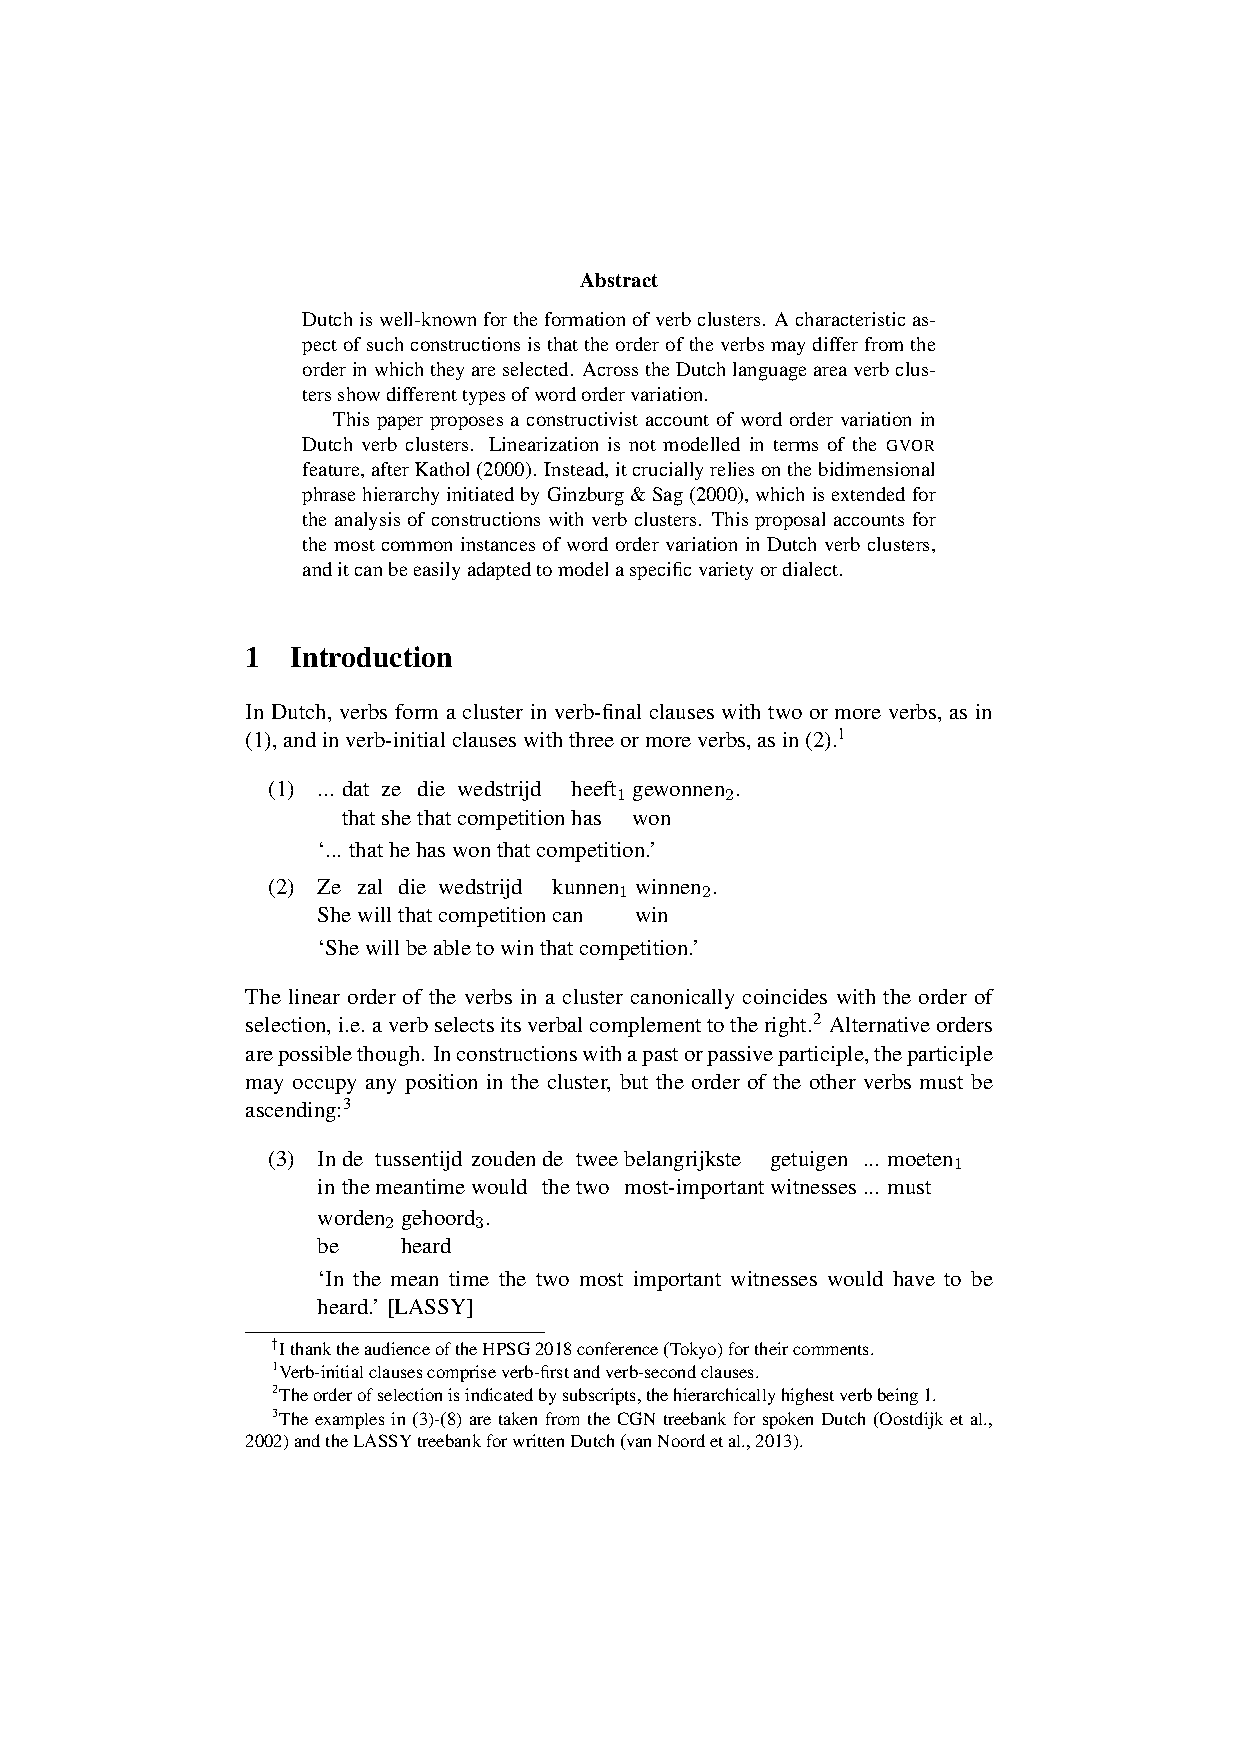
\includepdf[pages=-,pagecommand=\thispagestyle{plain}]{Includes/augustinus.pdf}
        \setcounter{page}{20}
        \phantomsection
        \addcontentsline{toc}{section}{Berthold Crysmann, Alain Kihm: Deriving reversal in  Old French nominal inflection}
\thispagestyle{empty}

\begin{center}
  {\huge\bfseries Deriving reversal in  Old French nominal inflection\par}

  \bigskip

~\\
\begingroup
\setlength{\leftskip}{0pt plus 1fill}
\setlength{\rightskip}{0pt plus 1fill}
\setlength{\parindent}{0pt}
\setlength{\parfillskip}{0pt}
  \formatauthor{Berthold Crysmann}{\begin{tabular}{@{}c@{}}CNRS, Laboratoire de linguistique formelle\end{tabular}}
\formatauthor{Alain Kihm}{\begin{tabular}{@{}c@{}}CNRS, Laboratoire de linguistique formelle\end{tabular}}

\par\endgroup

  \vspace*{8ex}

  Proceedings of the 25th International Conference on\par Head-Driven Phrase Structure Grammar

  \bigskip

  University of Tokyo

  \medskip

  Stefan  Müller, Frank Richter (Editors)

  \medskip

  2018

  \medskip

  CSLI Publications

  \medskip

  pages 20--35

  \medskip

  \url{http://csli-publications.stanford.edu/HPSG/2018}
\end{center}
\vfill

\noindent
Keywords: Morphological reversal,
Old French, Declension, HPSG, IbM, Overabundance


\vfill
\noindent
% APA Style
Crysmann, Berthold, \& Kihm, Alain. 2018. Deriving reversal in  Old French nominal inflection. In Müller, Stefan, \& Richter, Frank (Eds.), \emph{{Proceedings of the 25th International Conference on Head-Driven Phrase Structure Grammar, University of Tokyo}}, 20--35. Stanford,
CA: CSLI Publications. \hfill\href{http://creativecommons.org/licenses/by/4.0/}{
\includegraphics[height=.75em]{Includes/ccby-eps-converted-to.pdf}}

\newpage
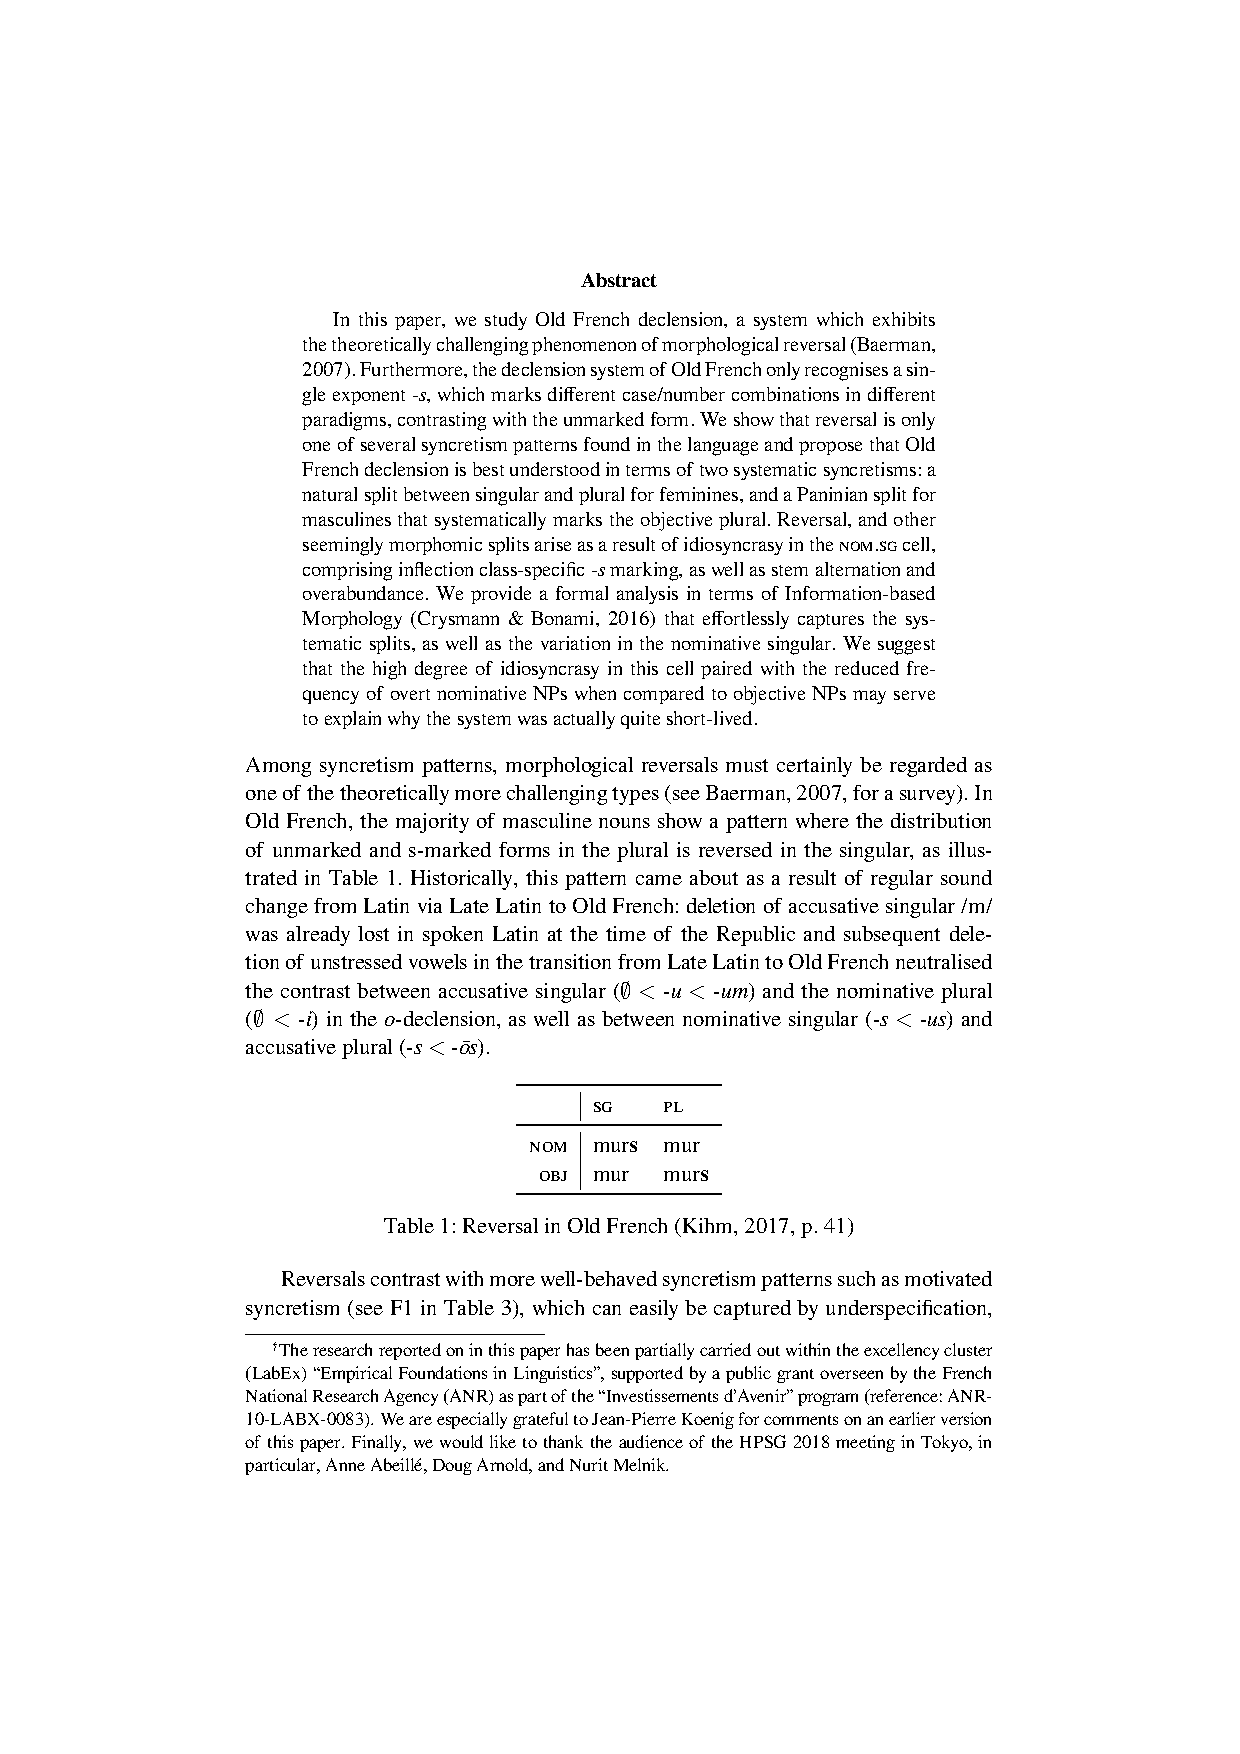
\includepdf[pages=-,pagecommand=\thispagestyle{plain}]{Includes/crysmann-kihm.pdf}
        \setcounter{page}{36}
        \phantomsection
        \addcontentsline{toc}{section}{Christian M. Curtis: Valence-changing morphology via lexical rule composition}
\thispagestyle{empty}

\begin{center}
  {\huge\bfseries Valence-changing morphology via lexical rule composition\par}

  \bigskip

~\\
\begingroup
\setlength{\leftskip}{0pt plus 1fill}
\setlength{\rightskip}{0pt plus 1fill}
\setlength{\parindent}{0pt}
\setlength{\parfillskip}{0pt}
  \formatauthor{Christian M. Curtis}{\begin{tabular}{@{}c@{}}University of Washington\end{tabular}}

\par\endgroup

  \vspace*{8ex}

  Proceedings of the 25th International Conference on\par Head-Driven Phrase Structure Grammar

  \bigskip

  University of Tokyo

  \medskip

  Stefan  Müller, Frank Richter (Editors)

  \medskip

  2018

  \medskip

  CSLI Publications

  \medskip

  pages 36--48

  \medskip

  \url{http://csli-publications.stanford.edu/HPSG/2018}
\end{center}
\vfill

\noindent
Keywords: HPSG, Valence Change, Grammar Matrix


\vfill
\noindent
% APA Style
Curtis, Christian M. 2018. Valence-changing morphology via lexical rule composition. In Müller, Stefan, \& Richter, Frank (Eds.), \emph{{Proceedings of the 25th International Conference on Head-Driven Phrase Structure Grammar, University of Tokyo}}, 36--48. Stanford,
CA: CSLI Publications. \hfill\href{http://creativecommons.org/licenses/by/4.0/}{
\includegraphics[height=.75em]{Includes/ccby-eps-converted-to.pdf}}

\newpage
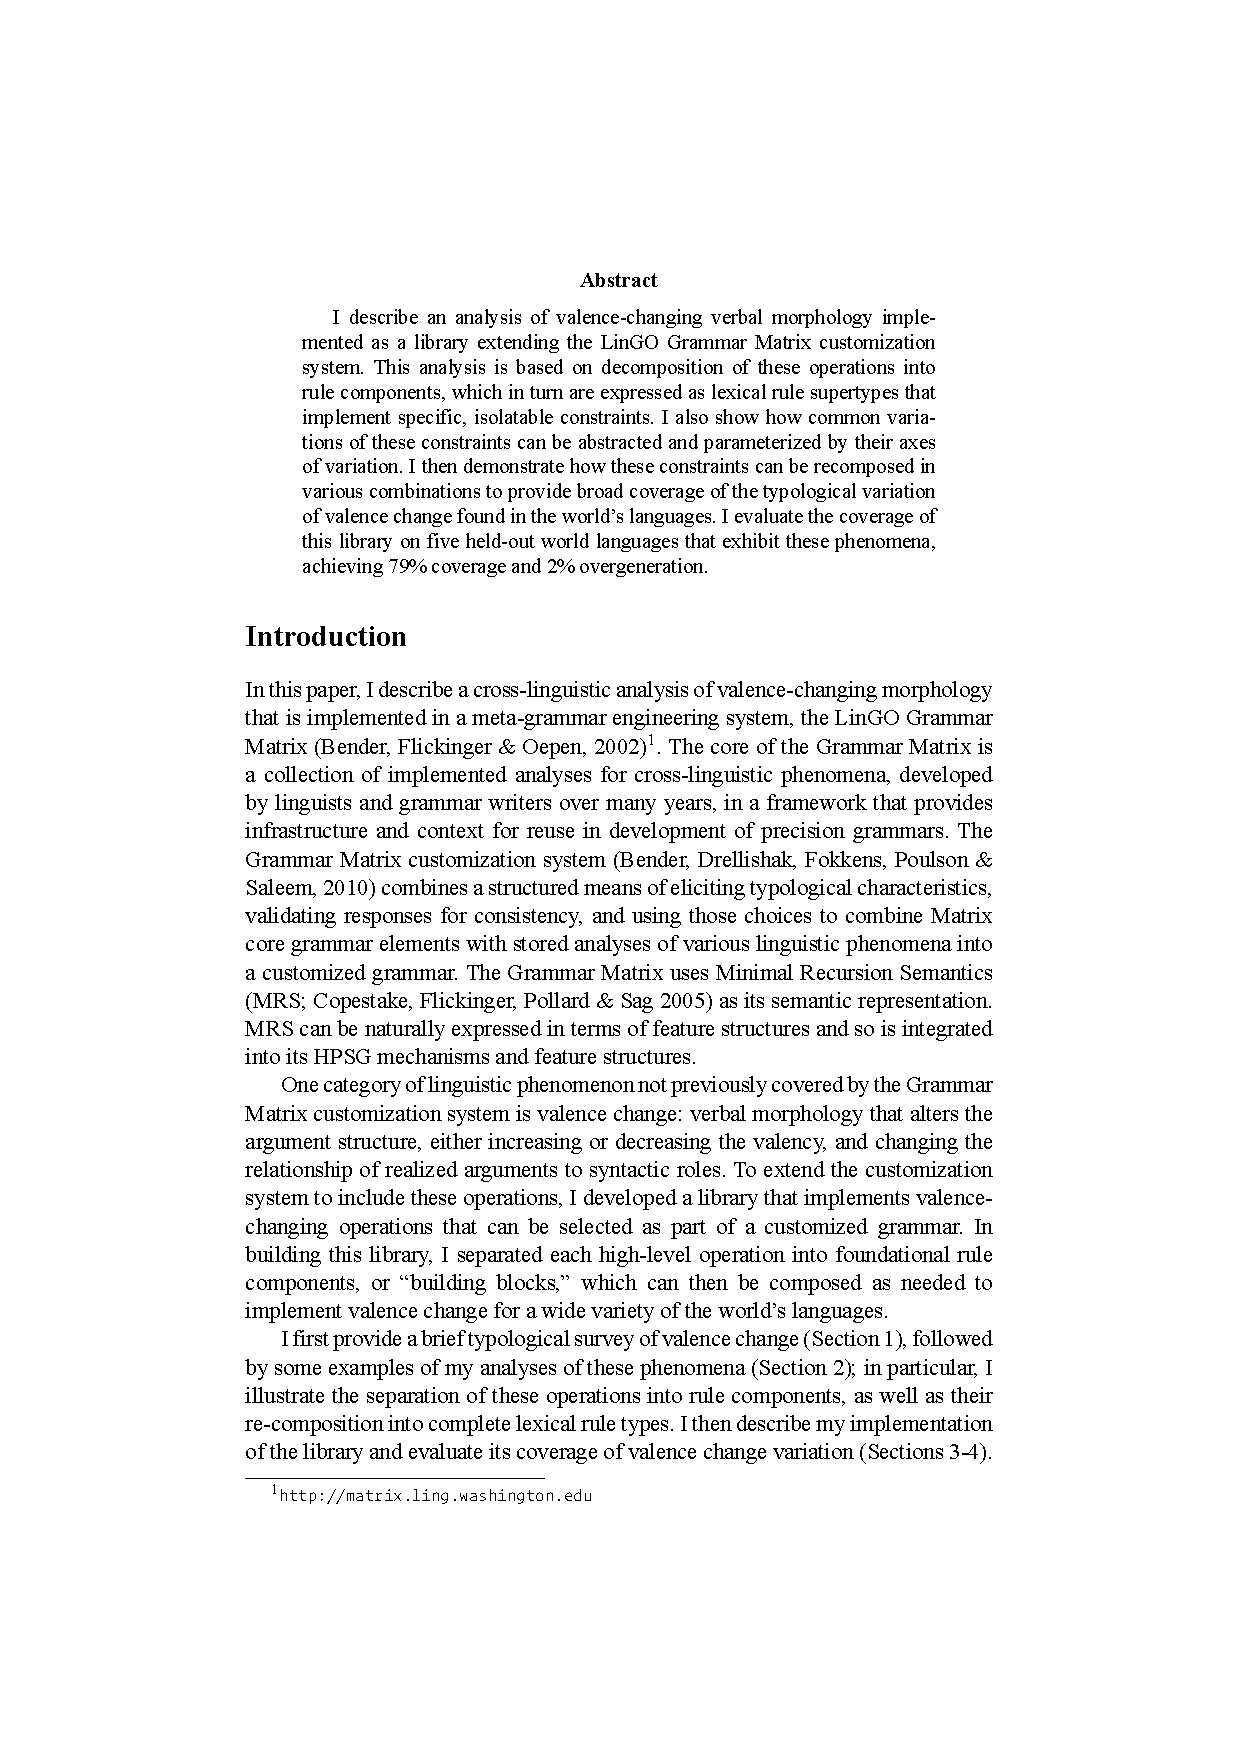
\includepdf[pages=-,pagecommand=\thispagestyle{plain}]{Includes/curtis.pdf}
        \setcounter{page}{49}
        \phantomsection
        \addcontentsline{toc}{section}{Anke Holler, Markus Steinbach: Sign language agreement:\\ A constraint-based perspective}
\thispagestyle{empty}

\begin{center}
  {\huge\bfseries Sign language agreement:\par A constraint-based perspective\par}

  \bigskip

~\\
\begingroup
\setlength{\leftskip}{0pt plus 1fill}
\setlength{\rightskip}{0pt plus 1fill}
\setlength{\parindent}{0pt}
\setlength{\parfillskip}{0pt}
  \formatauthor{Anke Holler}{\begin{tabular}{@{}c@{}}University of Göttingen\end{tabular}}
\formatauthor{Markus Steinbach}{\begin{tabular}{@{}c@{}}University of Göttingen\end{tabular}}

\par\endgroup

  \vspace*{8ex}

  Proceedings of the 25th International Conference on\par Head-Driven Phrase Structure Grammar

  \bigskip

  University of Tokyo

  \medskip

  Stefan  Müller, Frank Richter (Editors)

  \medskip

  2018

  \medskip

  CSLI Publications

  \medskip

  pages 49--65

  \medskip

  \url{http://csli-publications.stanford.edu/HPSG/2018}
\end{center}
\vfill

\noindent
Keywords: HPSG, DGS, Agreement, PAM


\vfill
\noindent
% APA Style
Holler, Anke, \& Steinbach, Markus. 2018. Sign language agreement:  A constraint-based perspective. In Müller, Stefan, \& Richter, Frank (Eds.), \emph{{Proceedings of the 25th International Conference on Head-Driven Phrase Structure Grammar, University of Tokyo}}, 49--65. Stanford,
CA: CSLI Publications. \hfill\href{http://creativecommons.org/licenses/by/4.0/}{
\includegraphics[height=.75em]{Includes/ccby-eps-converted-to.pdf}}

\newpage
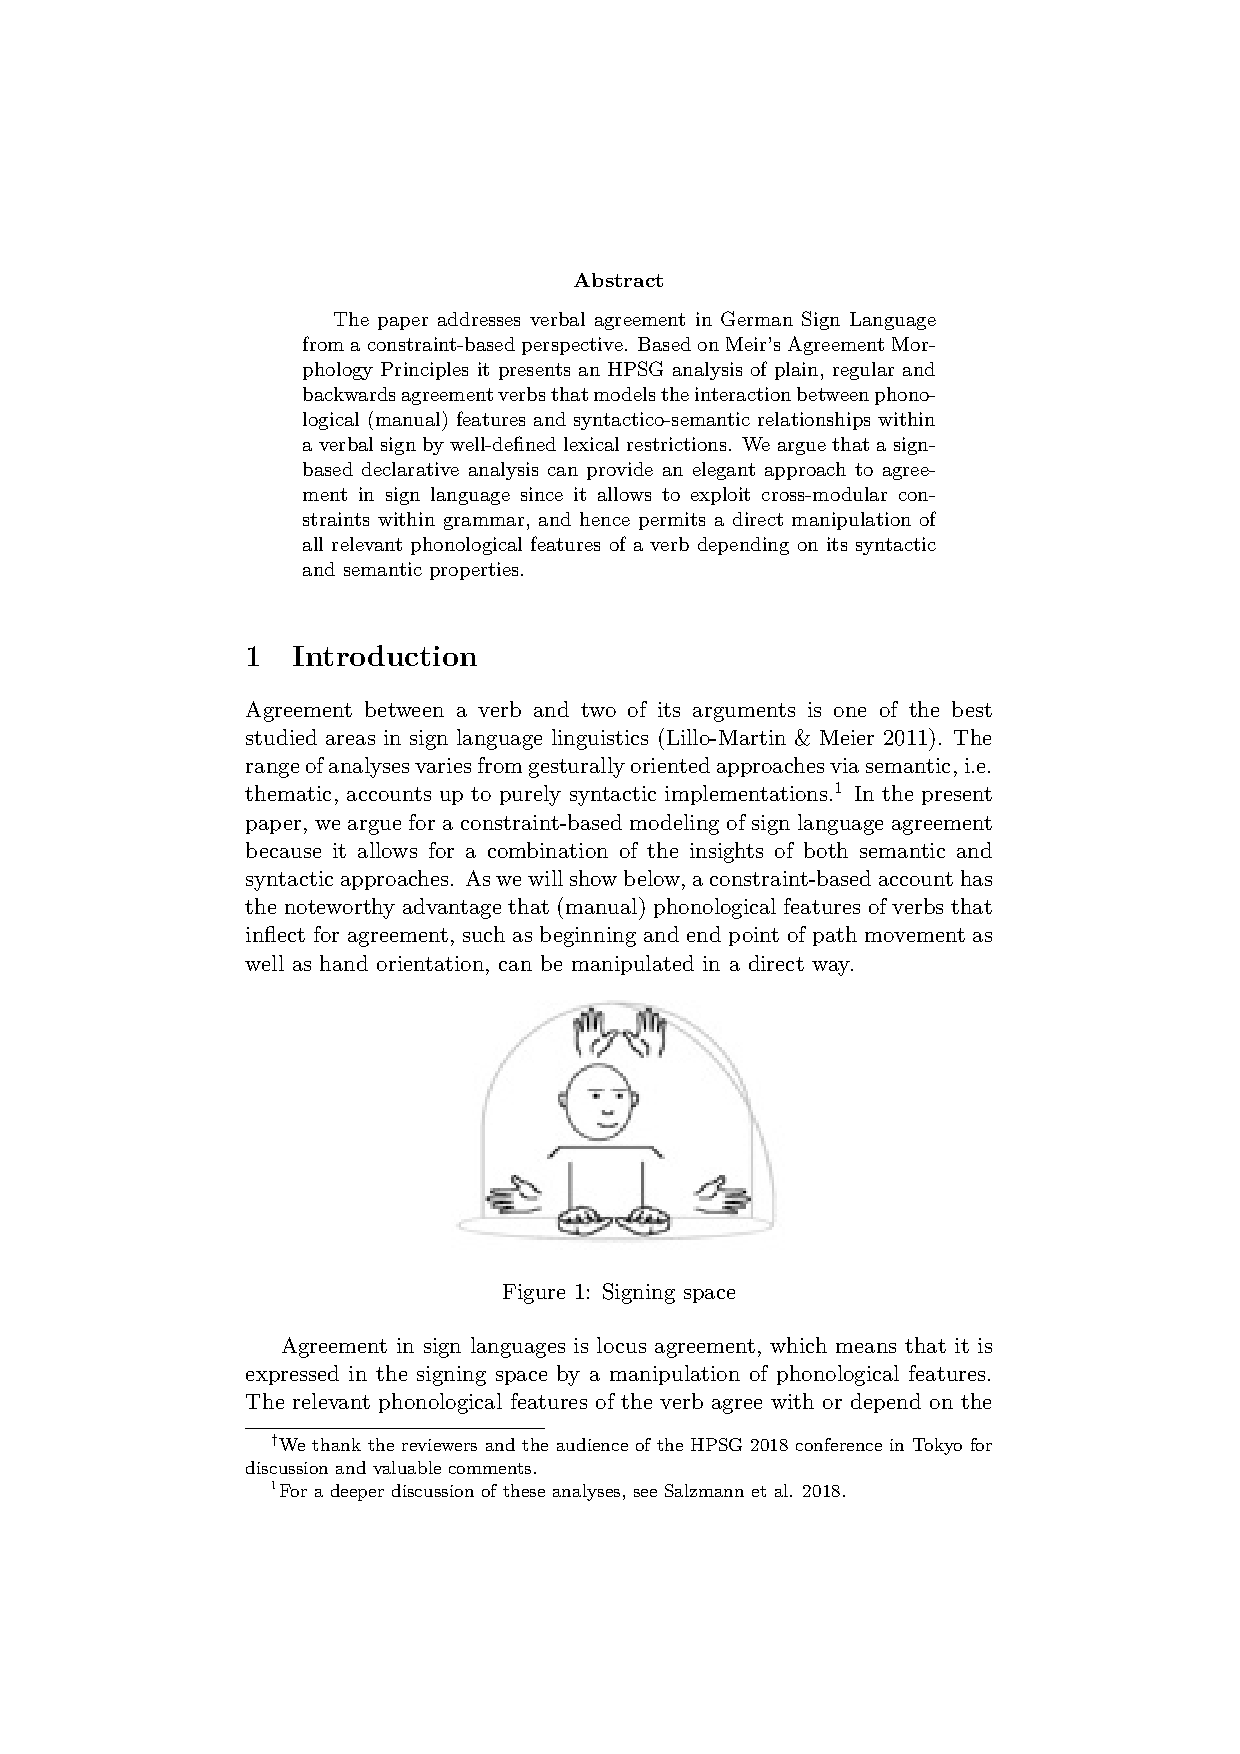
\includepdf[pages=-,pagecommand=\thispagestyle{plain}]{Includes/holler-steinbach.pdf}
        \setcounter{page}{66}
        \phantomsection
        \addcontentsline{toc}{section}{Kristen Howell, Olga Zamaraeva, Emily M. Bender: Nominalized Clauses in the Grammar Matrix}
\thispagestyle{empty}

\begin{center}
  {\huge\bfseries Nominalized Clauses in the Grammar Matrix\par}

  \bigskip

~\\
\begingroup
\setlength{\leftskip}{0pt plus 1fill}
\setlength{\rightskip}{0pt plus 1fill}
\setlength{\parindent}{0pt}
\setlength{\parfillskip}{0pt}
  \formatauthor{Kristen Howell}{\begin{tabular}{@{}c@{}}University of Washington\end{tabular}}
\formatauthor{Olga Zamaraeva}{\begin{tabular}{@{}c@{}}University of Washington\end{tabular}}
\formatauthor{Emily M. Bender}{\begin{tabular}{@{}c@{}}University of Washington\end{tabular}}

\par\endgroup

  \vspace*{8ex}

  Proceedings of the 25th International Conference on\par Head-Driven Phrase Structure Grammar

  \bigskip

  University of Tokyo

  \medskip

  Stefan  Müller, Frank Richter (Editors)

  \medskip

  2018

  \medskip

  CSLI Publications

  \medskip

  pages 66--86

  \medskip

  \url{http://csli-publications.stanford.edu/HPSG/2018}
\end{center}
\vfill

\noindent
Keywords: HPSG, Typology, Grammar Engineering, Nominalized clauses, Nominalization, Grammar Matrix


\vfill
\noindent
% APA Style
Howell, Kristen, Zamaraeva, Olga, \& Bender, Emily M. 2018. Nominalized Clauses in the Grammar Matrix. In Müller, Stefan, \& Richter, Frank (Eds.), \emph{{Proceedings of the 25th International Conference on Head-Driven Phrase Structure Grammar, University of Tokyo}}, 66--86. Stanford,
CA: CSLI Publications. \hfill\href{http://creativecommons.org/licenses/by/4.0/}{
\includegraphics[height=.75em]{Includes/ccby-eps-converted-to.pdf}}

\newpage
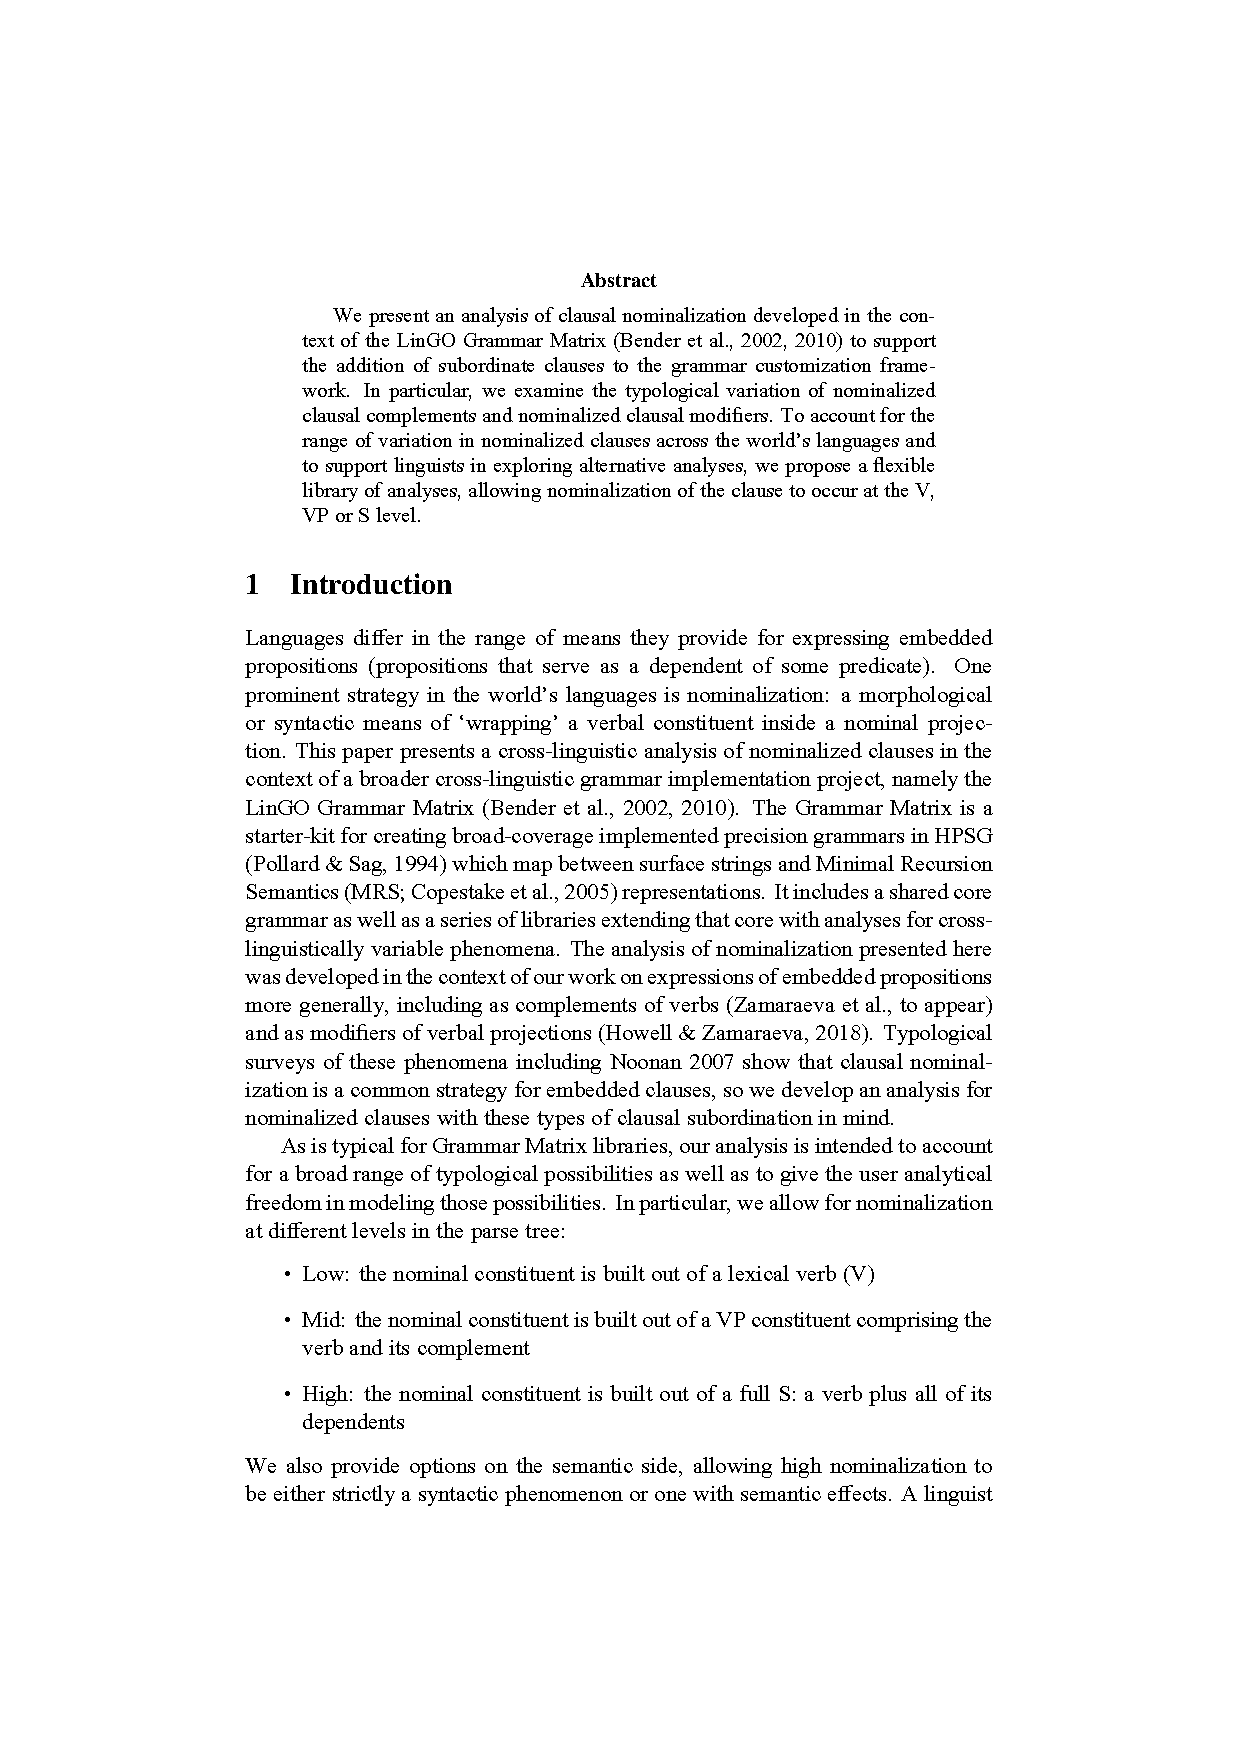
\includepdf[pages=-,pagecommand=\thispagestyle{plain}]{Includes/hzb.pdf}
        \setcounter{page}{87}
        \phantomsection
        \addcontentsline{toc}{section}{David Lahm: Plural in Lexical Resource
Semantics}
\thispagestyle{empty}

\begin{center}
  {\huge\bfseries Plural in Lexical Resource
Semantics\par}

  \bigskip

~\\
\begingroup
\setlength{\leftskip}{0pt plus 1fill}
\setlength{\rightskip}{0pt plus 1fill}
\setlength{\parindent}{0pt}
\setlength{\parfillskip}{0pt}
  \formatauthor{David Lahm}{\begin{tabular}{@{}c@{}}University of Frankfurt\end{tabular}}

\par\endgroup

  \vspace*{8ex}

  Proceedings of the 25th International Conference on\par Head-Driven Phrase Structure Grammar

  \bigskip

  University of Tokyo

  \medskip

  Stefan  Müller, Frank Richter (Editors)

  \medskip

  2018

  \medskip

  CSLI Publications

  \medskip

  pages 87--107

  \medskip

  \url{http://csli-publications.stanford.edu/HPSG/2018}
\end{center}
\vfill

\noindent
Keywords: plural, lexical resource semantics,
cumulation, cumulative predication, polyadic quantification,
underspecified semantics, semantic glue, maximalisation, covers


\vfill
\noindent
% APA Style
Lahm, David. 2018. Plural in Lexical Resource
Semantics. In Müller, Stefan, \& Richter, Frank (Eds.), \emph{{Proceedings of the 25th International Conference on Head-Driven Phrase Structure Grammar, University of Tokyo}}, 87--107. Stanford,
CA: CSLI Publications. \hfill\href{http://creativecommons.org/licenses/by/4.0/}{
\includegraphics[height=.75em]{Includes/ccby-eps-converted-to.pdf}}

\newpage
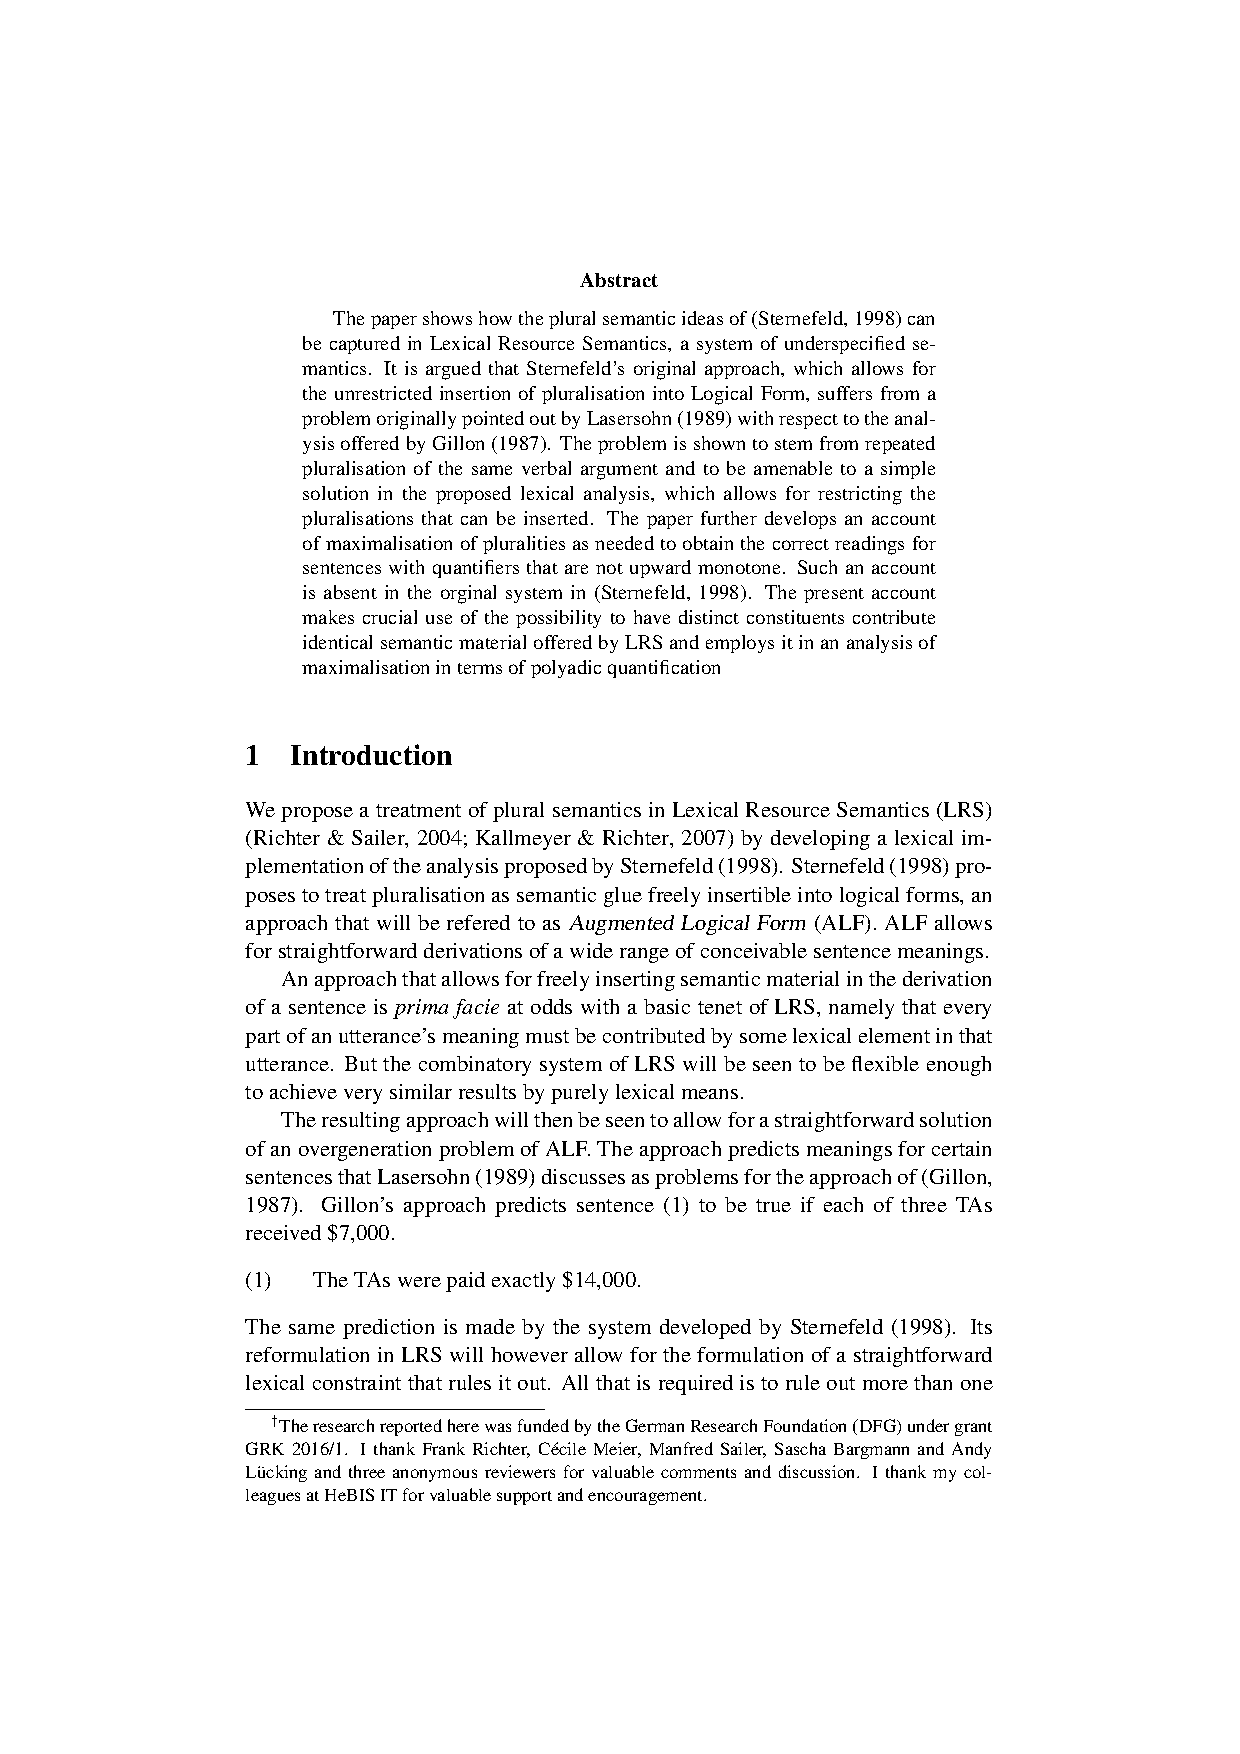
\includepdf[pages=-,pagecommand=\thispagestyle{plain}]{Includes/lahm.pdf}
        \setcounter{page}{108}
        \phantomsection
        \addcontentsline{toc}{section}{Nurit Melnik: Symmetry and asymmetry in the Hebrew copula construction}
\thispagestyle{empty}

\begin{center}
  {\huge\bfseries Symmetry and asymmetry in the Hebrew copula construction\par}

  \bigskip

~\\
\begingroup
\setlength{\leftskip}{0pt plus 1fill}
\setlength{\rightskip}{0pt plus 1fill}
\setlength{\parindent}{0pt}
\setlength{\parfillskip}{0pt}
  \formatauthor{Nurit Melnik}{\begin{tabular}{@{}c@{}}The Open University of Israel\end{tabular}}

\par\endgroup

  \vspace*{8ex}

  Proceedings of the 25th International Conference on\par Head-Driven Phrase Structure Grammar

  \bigskip

  University of Tokyo

  \medskip

  Stefan  Müller, Frank Richter (Editors)

  \medskip

  2018

  \medskip

  CSLI Publications

  \medskip

  pages 108--126

  \medskip

  \url{http://csli-publications.stanford.edu/HPSG/2018}
\end{center}
\vfill

\noindent
Keywords: HPSG, copula, agreement, inversion, Information Structure, Hebrew


\vfill
\noindent
% APA Style
Melnik, Nurit. 2018. Symmetry and asymmetry in the Hebrew copula construction. In Müller, Stefan, \& Richter, Frank (Eds.), \emph{{Proceedings of the 25th International Conference on Head-Driven Phrase Structure Grammar, University of Tokyo}}, 108--126. Stanford,
CA: CSLI Publications. \hfill\href{http://creativecommons.org/licenses/by/4.0/}{
\includegraphics[height=.75em]{Includes/ccby-eps-converted-to.pdf}}

\newpage
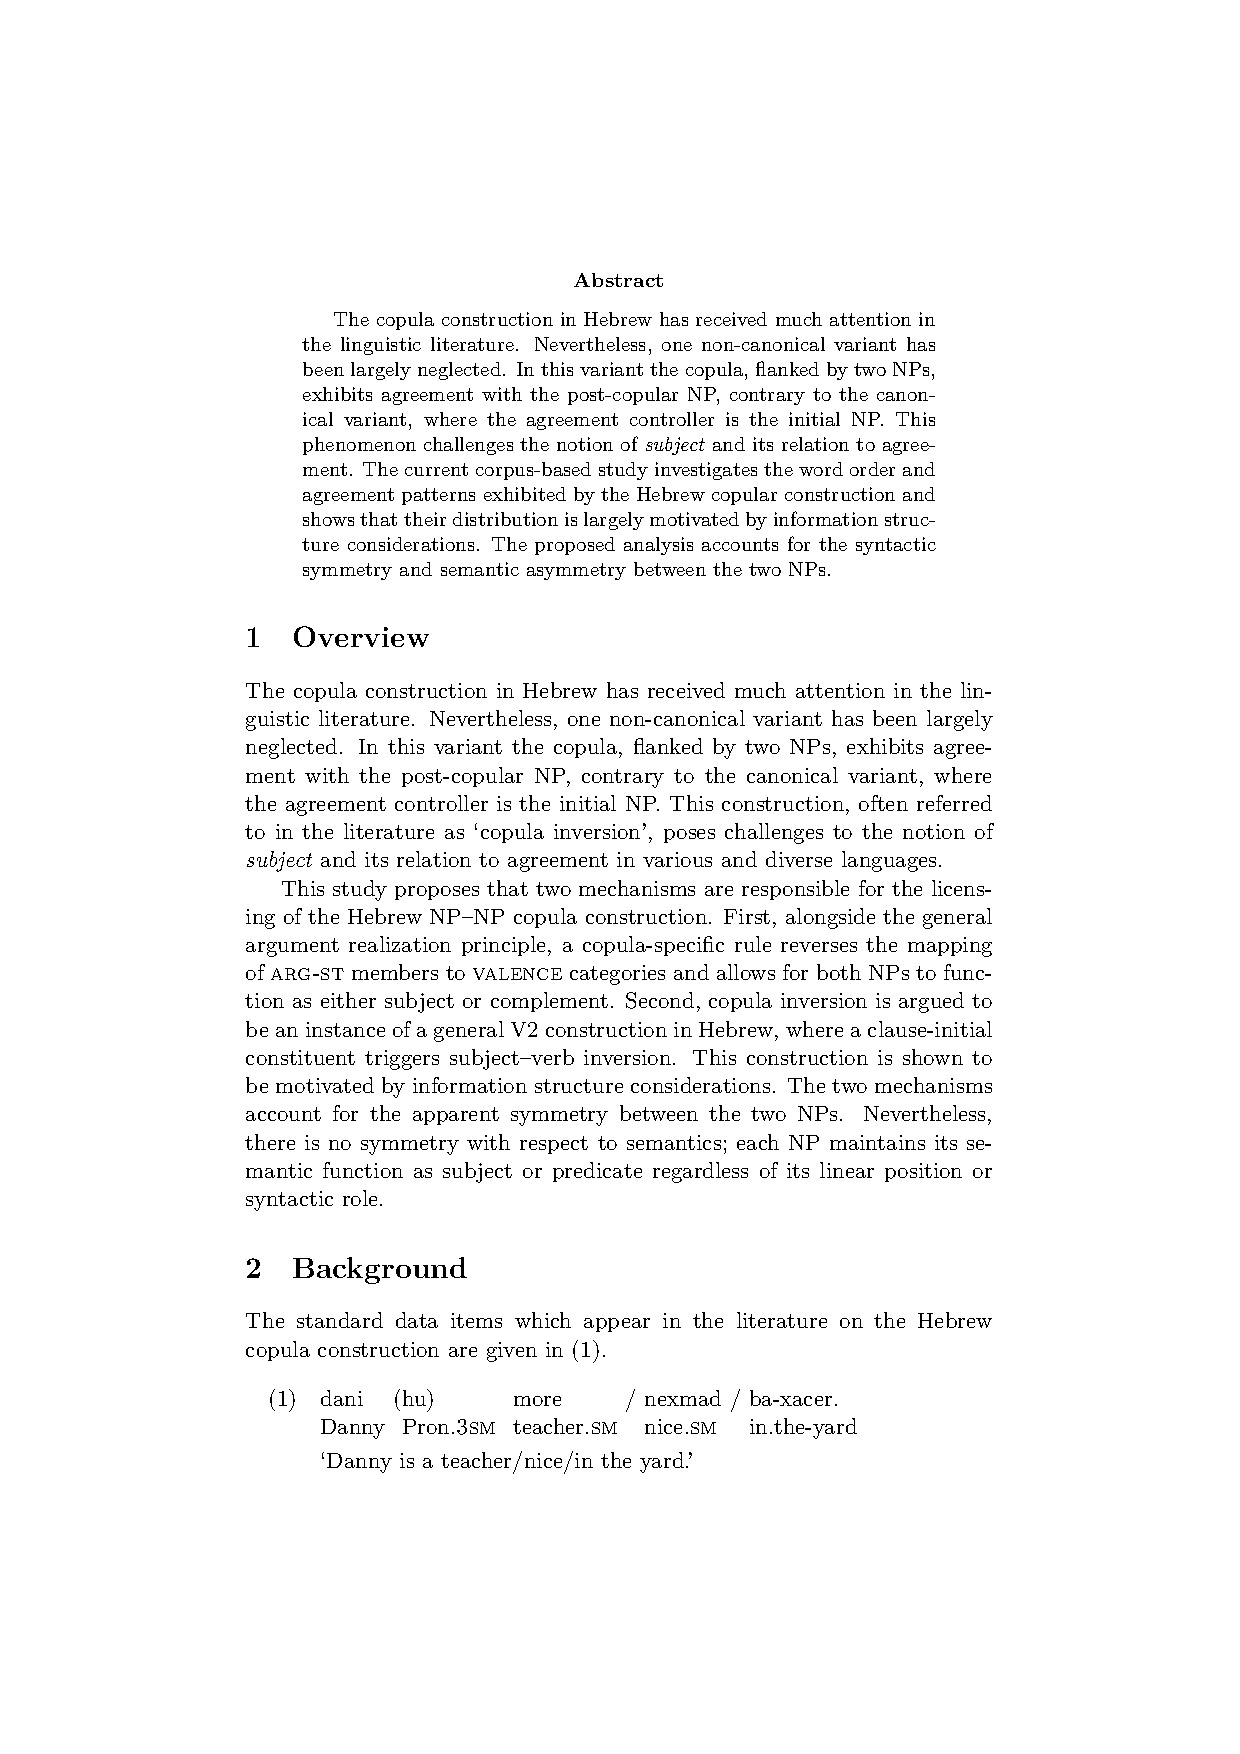
\includepdf[pages=-,pagecommand=\thispagestyle{plain}]{Includes/melnik.pdf}
        \setcounter{page}{127}
        \phantomsection
        \addcontentsline{toc}{section}{David Moeljadi, Francis Bond: HPSG Analysis and Computational Implementation of Indonesian Passives}
\thispagestyle{empty}

\begin{center}
  {\huge\bfseries HPSG Analysis and Computational Implementation of Indonesian Passives\par}

  \bigskip

~\\
\begingroup
\setlength{\leftskip}{0pt plus 1fill}
\setlength{\rightskip}{0pt plus 1fill}
\setlength{\parindent}{0pt}
\setlength{\parfillskip}{0pt}
  \formatauthor{David Moeljadi}{\begin{tabular}{@{}c@{}}Nanyang Technological University\end{tabular}}
\formatauthor{Francis Bond}{\begin{tabular}{@{}c@{}}Nanyang Technological University\end{tabular}}

\par\endgroup

  \vspace*{8ex}

  Proceedings of the 25th International Conference on\par Head-Driven Phrase Structure Grammar

  \bigskip

  University of Tokyo

  \medskip

  Stefan  Müller, Frank Richter (Editors)

  \medskip

  2018

  \medskip

  CSLI Publications

  \medskip

  pages 127--137

  \medskip

  \url{http://csli-publications.stanford.edu/HPSG/2018}
\end{center}
\vfill

\noindent
Keywords: HPSG, Indonesian, passives, INDRA


\vfill
\noindent
% APA Style
Moeljadi, David, \& Bond, Francis. 2018. HPSG Analysis and Computational Implementation of Indonesian Passives. In Müller, Stefan, \& Richter, Frank (Eds.), \emph{{Proceedings of the 25th International Conference on Head-Driven Phrase Structure Grammar, University of Tokyo}}, 127--137. Stanford,
CA: CSLI Publications. \hfill\href{http://creativecommons.org/licenses/by/4.0/}{
\includegraphics[height=.75em]{Includes/ccby-eps-converted-to.pdf}}

\newpage
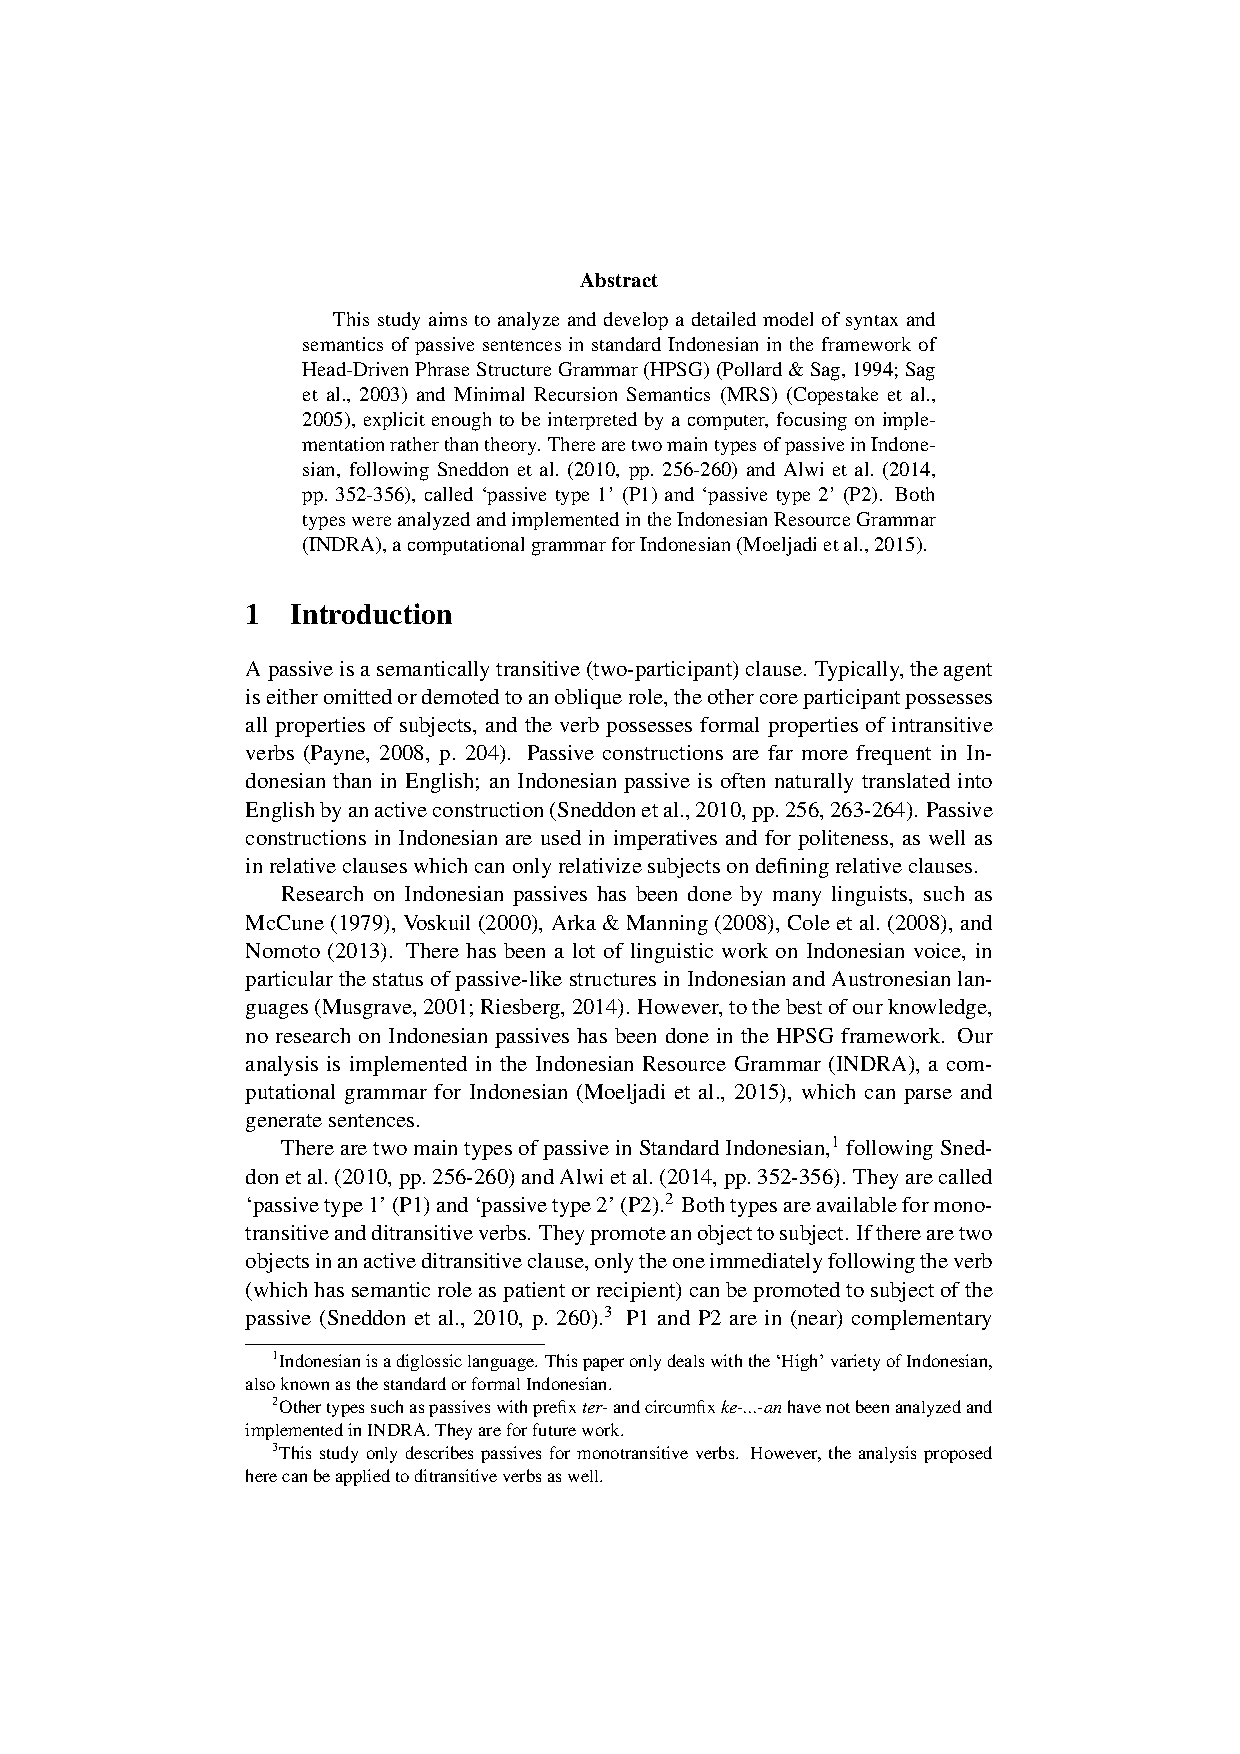
\includepdf[pages=-,pagecommand=\thispagestyle{plain}]{Includes/moeljadi-bond.pdf}
        \setcounter{page}{138}
        \phantomsection
        \addcontentsline{toc}{section}{Elizabeth Nielsen, Emily M. Bender: Modeling Adnominal Possession in Multilingual Grammar Engineering}
\thispagestyle{empty}

\begin{center}
  {\huge\bfseries Modeling Adnominal Possession in Multilingual Grammar Engineering\par}

  \bigskip

~\\
\begingroup
\setlength{\leftskip}{0pt plus 1fill}
\setlength{\rightskip}{0pt plus 1fill}
\setlength{\parindent}{0pt}
\setlength{\parfillskip}{0pt}
  \formatauthor{Elizabeth Nielsen}{\begin{tabular}{@{}c@{}}University of Washington\end{tabular}}
\formatauthor{Emily M. Bender}{\begin{tabular}{@{}c@{}}University of Washington\end{tabular}}

\par\endgroup

  \vspace*{8ex}

  Proceedings of the 25th International Conference on\par Head-Driven Phrase Structure Grammar

  \bigskip

  University of Tokyo

  \medskip

  Stefan  Müller, Frank Richter (Editors)

  \medskip

  2018

  \medskip

  CSLI Publications

  \medskip

  pages 138--151

  \medskip

  \url{http://csli-publications.stanford.edu/HPSG/2018}
\end{center}
\vfill

\noindent
Keywords: adnominal possession, grammar engineering, computational typology, Grammar Matrix


\vfill
\noindent
% APA Style
Nielsen, Elizabeth, \& Bender, Emily M. 2018. Modeling Adnominal Possession in Multilingual Grammar Engineering. In Müller, Stefan, \& Richter, Frank (Eds.), \emph{{Proceedings of the 25th International Conference on Head-Driven Phrase Structure Grammar, University of Tokyo}}, 138--151. Stanford,
CA: CSLI Publications. \hfill\href{http://creativecommons.org/licenses/by/4.0/}{
\includegraphics[height=.75em]{Includes/ccby-eps-converted-to.pdf}}

\newpage
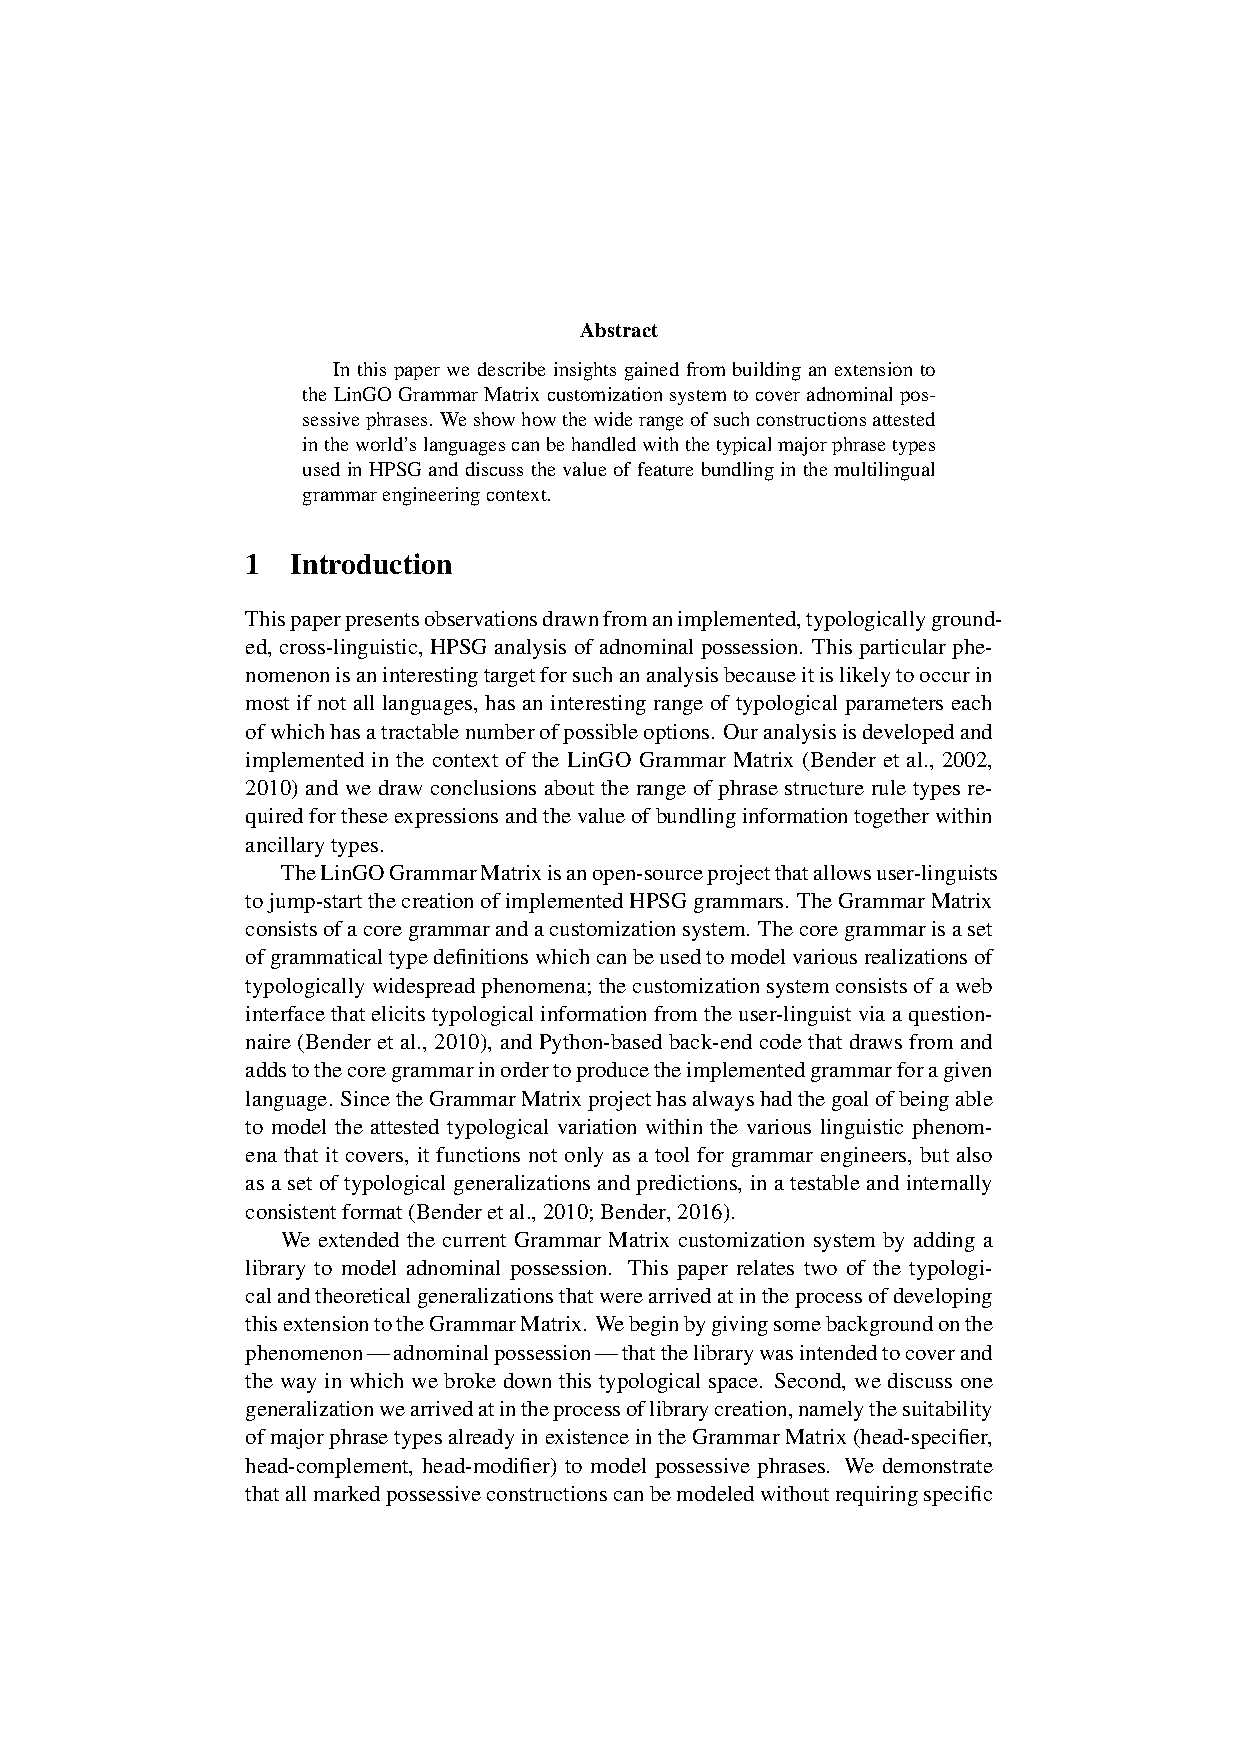
\includepdf[pages=-,pagecommand=\thispagestyle{plain}]{Includes/nielsen-bender.pdf}
\part{Contributions to the Workshop}
\thispagestyle{empty}
\newpage
        \setcounter{page}{153}
        \phantomsection
        \addcontentsline{toc}{section}{Antonio Machicao y Priemer, Paola Fritz-Huechante: Korean and Spanish psych-verbs: Interaction of case, theta-roles, linearization, and event structure in HPSG}
\thispagestyle{empty}

\begin{center}
  {\huge\bfseries Korean and Spanish psych-verbs: Interaction of case, theta-roles, linearization, and event structure in HPSG\par}

  \bigskip

~\\
\begingroup
\setlength{\leftskip}{0pt plus 1fill}
\setlength{\rightskip}{0pt plus 1fill}
\setlength{\parindent}{0pt}
\setlength{\parfillskip}{0pt}
  \formatauthor{Antonio Machicao y Priemer}{\begin{tabular}{@{}c@{}}Humboldt-Universität zu Berlin\end{tabular}}
\formatauthor{Paola Fritz-Huechante}{\begin{tabular}{@{}c@{}}Humboldt-Universität zu Berlin\end{tabular}}

\par\endgroup

  \vspace*{8ex}

  Proceedings of the 25th International Conference on\par Head-Driven Phrase Structure Grammar

  \bigskip

  University of Tokyo

  \medskip

  Stefan  Müller, Frank Richter (Editors)

  \medskip

  2018

  \medskip

  CSLI Publications

  \medskip

  pages 153--173

  \medskip

  \url{http://csli-publications.stanford.edu/HPSG/2018}
\end{center}
\vfill

\noindent
Keywords: Spanish, Korean, Psych-Verbs, Theta-Roles, Neo-Davidsonian, Linking


\vfill
\noindent
% APA Style
Machicao y Priemer, Antonio, \& Fritz-Huechante, Paola. 2018. Korean and Spanish psych-verbs: Interaction of case, theta-roles, linearization, and event structure in HPSG. In Müller, Stefan, \& Richter, Frank (Eds.), \emph{{Proceedings of the 25th International Conference on Head-Driven Phrase Structure Grammar, University of Tokyo}}, 153--173. Stanford,
CA: CSLI Publications. \hfill\href{http://creativecommons.org/licenses/by/4.0/}{
\includegraphics[height=.75em]{Includes/ccby-eps-converted-to.pdf}}

\newpage
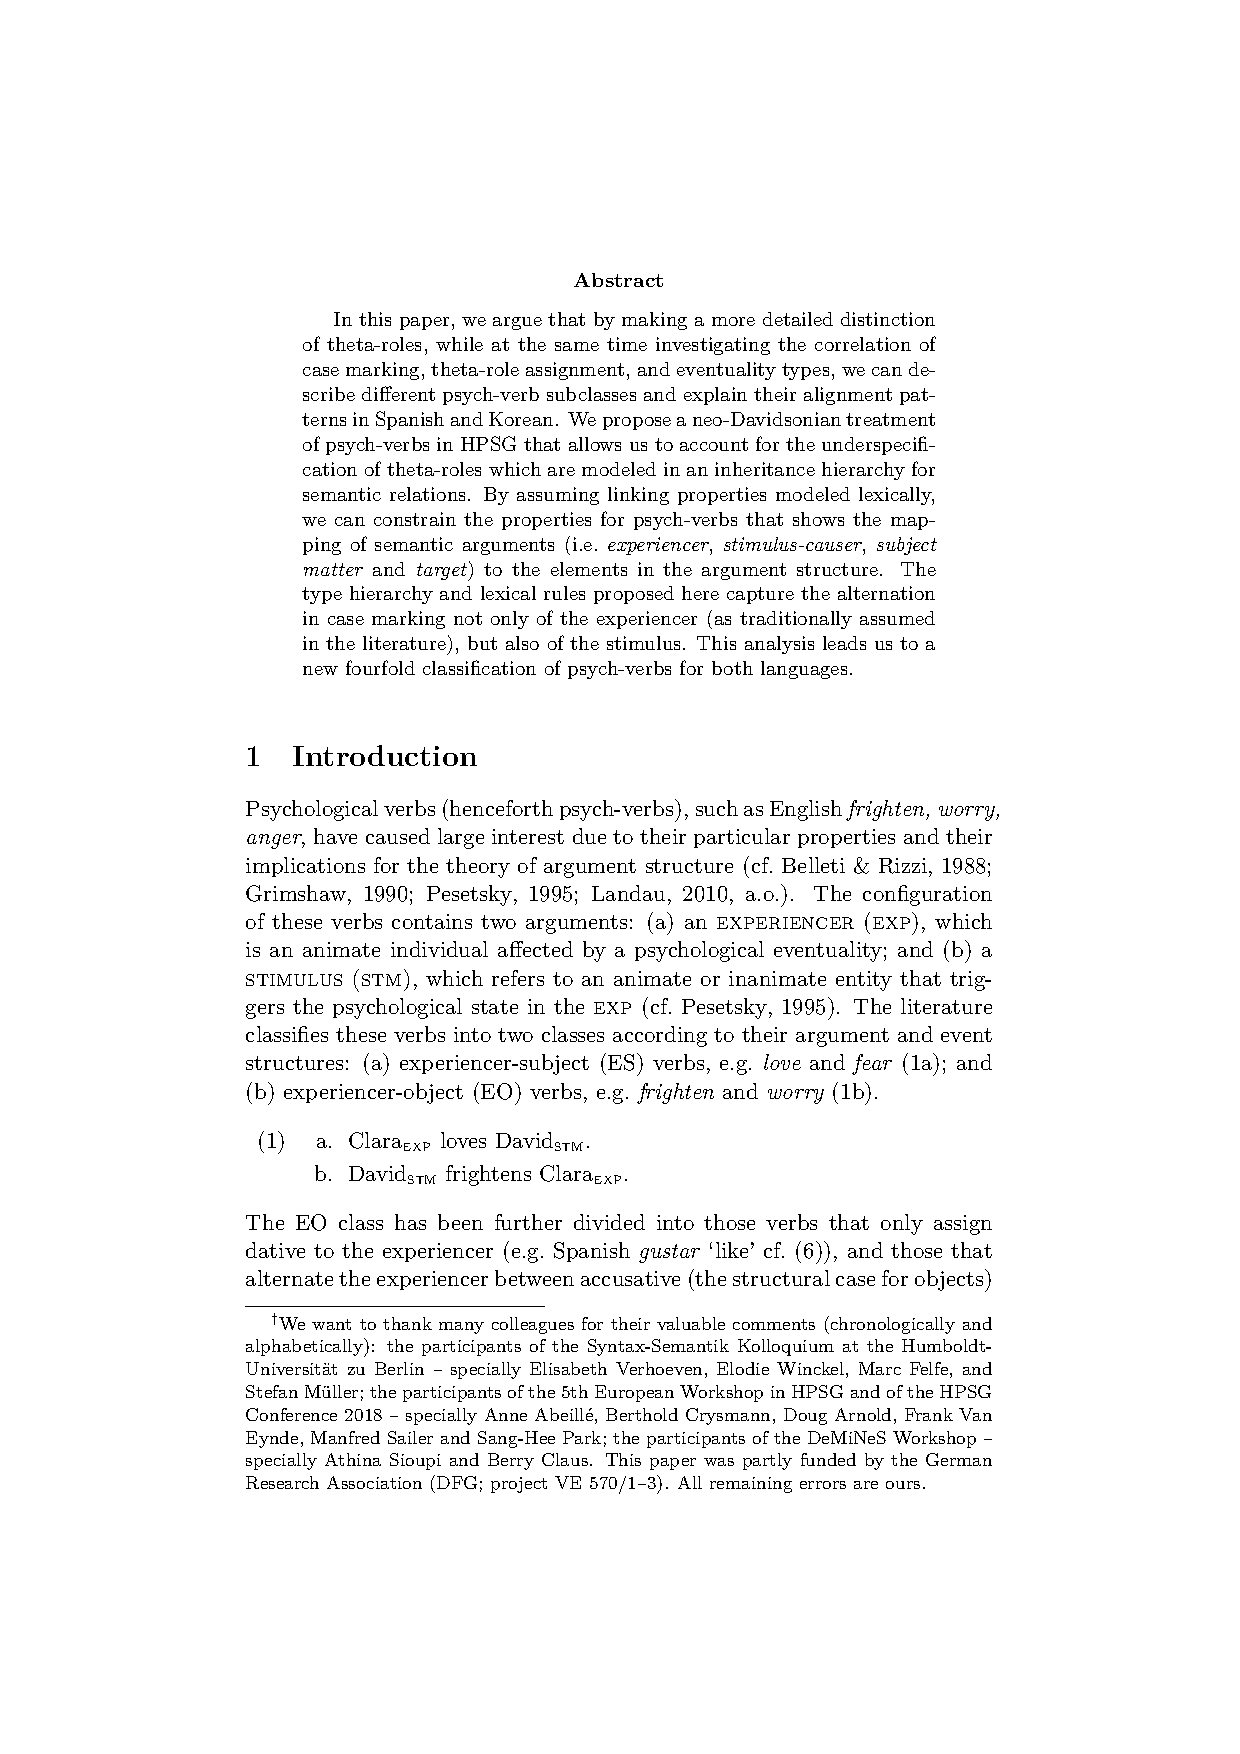
\includepdf[pages=-,pagecommand=\thispagestyle{plain}]{Includes/machicaoypriemer-fritz-huechante.pdf}
        \setcounter{page}{174}
        \phantomsection
        \addcontentsline{toc}{section}{Sh{\^u}ichi Yatabe, Kei Tanigawa: The fine structure of clausal right-node raising constructions in Japanese}
\thispagestyle{empty}

\begin{center}
  {\huge\bfseries The fine structure of clausal right-node raising constructions in Japanese\par}

  \bigskip

~\\
\begingroup
\setlength{\leftskip}{0pt plus 1fill}
\setlength{\rightskip}{0pt plus 1fill}
\setlength{\parindent}{0pt}
\setlength{\parfillskip}{0pt}
  \formatauthor{Shûichi Yatabe}{\begin{tabular}{@{}c@{}}University of Tokyo\end{tabular}}
\formatauthor{Kei Tanigawa}{\begin{tabular}{@{}c@{}}University of Tokyo\end{tabular}}

\par\endgroup

  \vspace*{8ex}

  Proceedings of the 25th International Conference on\par Head-Driven Phrase Structure Grammar

  \bigskip

  University of Tokyo

  \medskip

  Stefan  Müller, Frank Richter (Editors)

  \medskip

  2018

  \medskip

  CSLI Publications

  \medskip

  pages 174--194

  \medskip

  \url{http://csli-publications.stanford.edu/HPSG/2018}
\end{center}
\vfill

\noindent
Keywords: the lexicalist hypothesis, non-constituent coordination


\vfill
\noindent
% APA Style
Yatabe, Shûichi, \& Tanigawa, Kei. 2018. The fine structure of clausal right-node raising constructions in Japanese. In Müller, Stefan, \& Richter, Frank (Eds.), \emph{{Proceedings of the 25th International Conference on Head-Driven Phrase Structure Grammar, University of Tokyo}}, 174--194. Stanford,
CA: CSLI Publications. \hfill\href{http://creativecommons.org/licenses/by/4.0/}{
\includegraphics[height=.75em]{Includes/ccby-eps-converted-to.pdf}}

\newpage
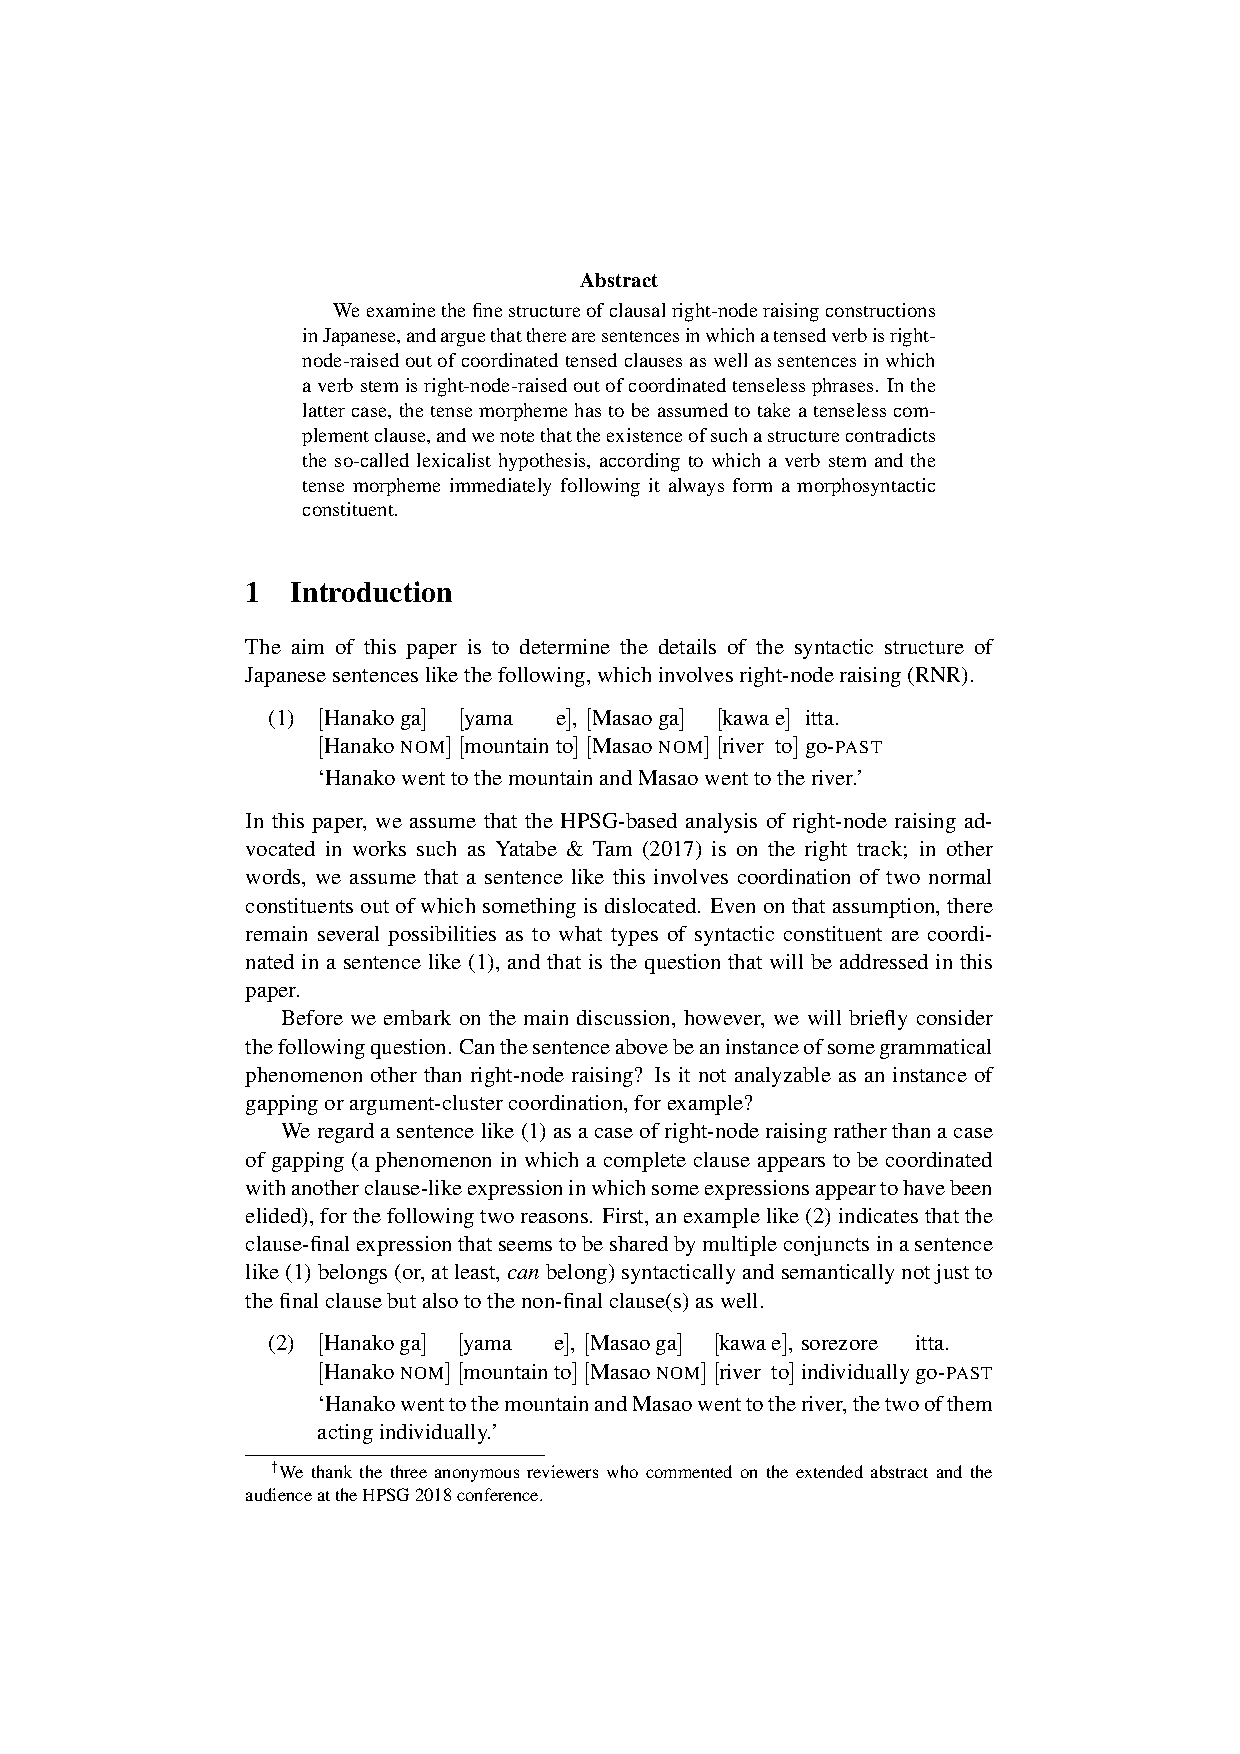
\includepdf[pages=-,pagecommand=\thispagestyle{plain}]{Includes/yatabe-tanigawa.pdf}
\end{document}
